Das L"osen von Eigenwertproblemen ist eine Standarddisziplin in der
numerischen linearen Algebra. Die konkrete Problemstellung dabei lautet: Zu gegebenen Matrizen $A,B\in\Cnn$ sollen Paare $(\lambda, x)$ mit $\lambda\in\C$ und $x\in\Co$ gefunden werden, welche
der Gleichung
\begin{equation}\label{eq:eigenproblem}
Ax = \lambda Bx
\end{equation}

gen"ugen. Solchen \emph{Eigenwertgleichungen} begegnet man in ganz unterschiedlichen Kontexten.
So sind sie beispielsweise bei der Bestimmung von Eigenfrequenzen oder dem Ermitteln von Fixpunkten beim
Rotieren eines Fu"sballs\footnote{Hier wird auf den bekannten
\emph{Satz vom Fu"sball} angespielt. Dieser besagt, dass auf einem Fußball
zwei Punkte existieren, die zu Spielbeginn und zur Halbzeit
an der gleichen Stelle liegen -- informell formuliert.} ebenso wie beim
Untersuchen des PageRanks\footnote{
Siehe Abschnitt zwei in ~\cite{page}.
} einer Website von
Bedeutung. Entsprechend strotz der Kanon von angebotenen numerischen
L"osungsmethoden von Vielfalt und Virtuosit"at.\footnote{Dies best"atigt sich beispielsweise bei einem Blick in das Inhaltsverzeichnis von ~\cite{stewart}.}\\

Nun mag der Fall eintreten, da es notwendig wird, lediglich eine Teilmenge
aus der Menge aller Eigenpaare zu untersuchen. Betrachten wir zur Illustration folgende Abbildung.

\begin{figure}[h!]\label{im:cat}
  \centering
  \resizebox{.4\linewidth}{!}{
\includegraphics{images/cat}}
  \caption{Katze mit Sonnenbrille (\copyright Andy Prokh).}
\end{figure}

Diese Foto ben"otigt in der Originalgr"o"se einen Speicherplatz von \textcolor{red}{9000mb}.\footnote{Das Foto aus Abbildung \ref{im:cat} wurde dabei mit einer \textcolor{red}{tollen Kamera} gemacht.}
Man stelle sich vor, man wolle dieses Bild komprimieren, um den ben"otigten Speicherplatz zu reduzieren.
Dies l"asst sich beispielsweise mit einer sogenannten \emph{Singul"arwertzerlegung} -- von Numerikern liebevoll als das \emph{Schweizer Taschenmesser der linearen Algebra} bezeichnet -- bewerkstelligen.\\

Da es sich bei Abbildung \ref{im:cat} um ein Schwarz-Wei"s-Bild handelt, l"asst sie sich als eine Matrix $M$ auffassen, deren Eintr"age die Grauwerte der einzelnen Pixel repr"asentieren.
Unter Anwendung des Satzes von der Singul"arwertzerlegung\footnote{Eine Formulierung ohne Beweis ist mit Satz \ref{thm:svd} -- zu finden im Anhang -- gegeben.} l"asst sich nun das Bild der Katze durch eine Folge von Matrizen niedrigeren Ranges approximieren.
Man berechnet hierf"ur die Wurzeln der von Null verschiedenen Eigenwerte von $M^H M$ und verwendet dann diese sogenannten \emph{Singul"arwerte} um die Matrix $M$ zu rekonstruieren.
Auf weitere Details "uber den hinter diesem Verfahren stehenden Algorithmus wollen wir an dieser Stelle verzichten.\\

Die Matrix $M$ hat in unserem Beispiel mehr als 700 Singul"arwerte. Die Frage ist nun, ob wir uns von einigen Singul"arwerten trennen k"onnen und dennoch eine akzeptable Bildqualit"at aufrecht erhalten k"onnen.
Insbesondere ist wichtig zu wissen, welche dieser Werte entscheidend f"ur die Rekonstruktion sind.\\

Dazu nehmen wir uns die $n\in\N$ Singul"arwerte $\sigma_1,\ldots,\sigma_n$ her. Ohne Einschr"ankung seien diese so nummeriert, dass $\sigma_1 \ge \ldots \ge \sigma_n$ gilt. Sollte dies nicht der Fall sein, nummerieren wir einfach um.
Nun filtern wir nach eigenen Kriterien Teilmengen aus den Singul"arwerten, beziehungsweise den Eigenwerten von $M^H M$ heraus und rekonstruieren mit deren Hilfe die Abbildung \ref{im:cat}.\\

Es sei an dieser Stelle darauf hingewiesen, dass die folgendenen Beurteilungen der Bildqualit"at nicht mathematisch begr"undet sind.
Die Eindr"ucke entstammen dem pers"onlichen Empfinden des Autors, sowie den Aussagen einer kleinen Testgruppe von Studierenden des Fachs Mathematik.\\

Beginnen wir mit einer mehr oder weniger willk"urlichen Auswahl von Singul"arwerten (SW).

\begin{figure}[h!]\label{im:cat:interval}
\center
\begin{subfigure}[c]{.3\textwidth}

\includegraphics[width=.9\linewidth]{images/cat10-30}
\subcaption{SW $\sigma_{10},\ldots,\sigma_{30}$.}
\end{subfigure}
\begin{subfigure}[c]{.3\textwidth}
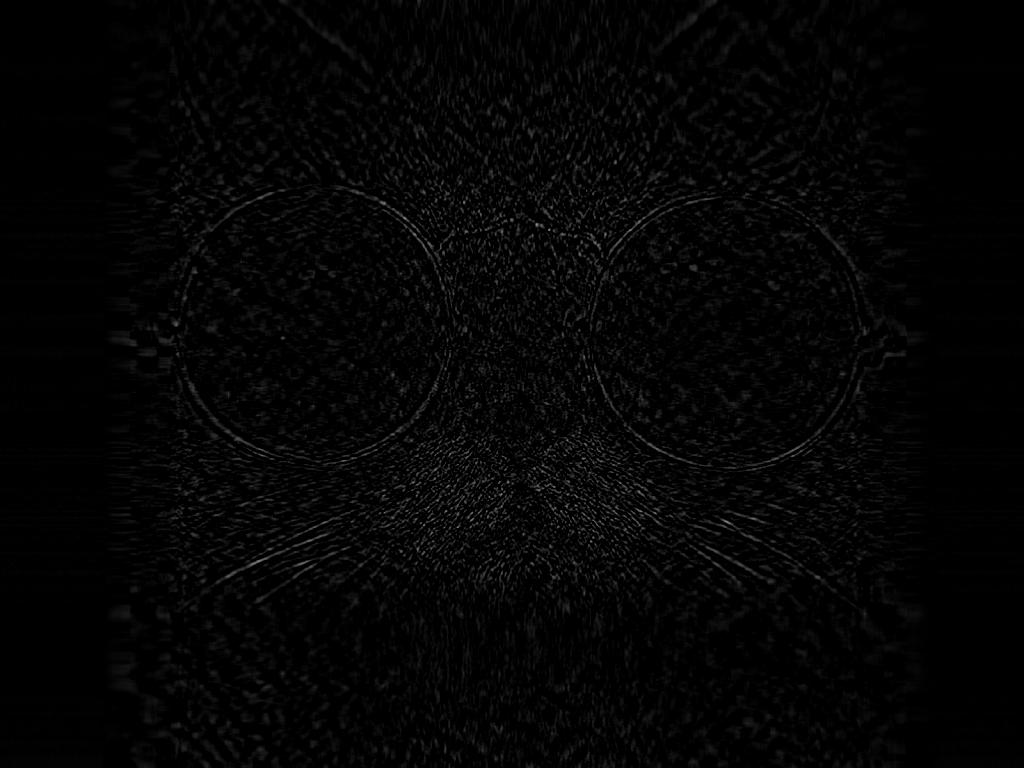
\includegraphics[width=.9\linewidth]{images/cat40-90}
\subcaption{SW $\sigma_{40},\ldots,\sigma_{90}$.}
\end{subfigure}
\begin{subfigure}[c]{.3\textwidth}

\includegraphics[width=.9\linewidth]{images/cat100-400}
\subcaption{SW $\sigma_{100},\ldots,\sigma_{400}$.}
\end{subfigure}

\caption{Rekonstruktion von Abbildung \ref{im:cat} mittels Singul"arwertzerlegung.}
\end{figure}

Die in Abbildung \ref{im:cat:interval} gew"ahlte Filtrierung erscheint etwas ungl"ucklich, da das urspr"ungliche Bild kaum wieder zu erkennen ist.
Versuchen wir unser Gl"uck daher mit einer anderen Wahl von Singul"arwerten.

\newpage

\begin{figure}[h!]
\center
\begin{subfigure}[c]{.3\textwidth}

\includegraphics[width=.9\linewidth]{images/cat1}
\subcaption{SW $\sigma_1$.}
\end{subfigure}
\begin{subfigure}[c]{.3\textwidth}
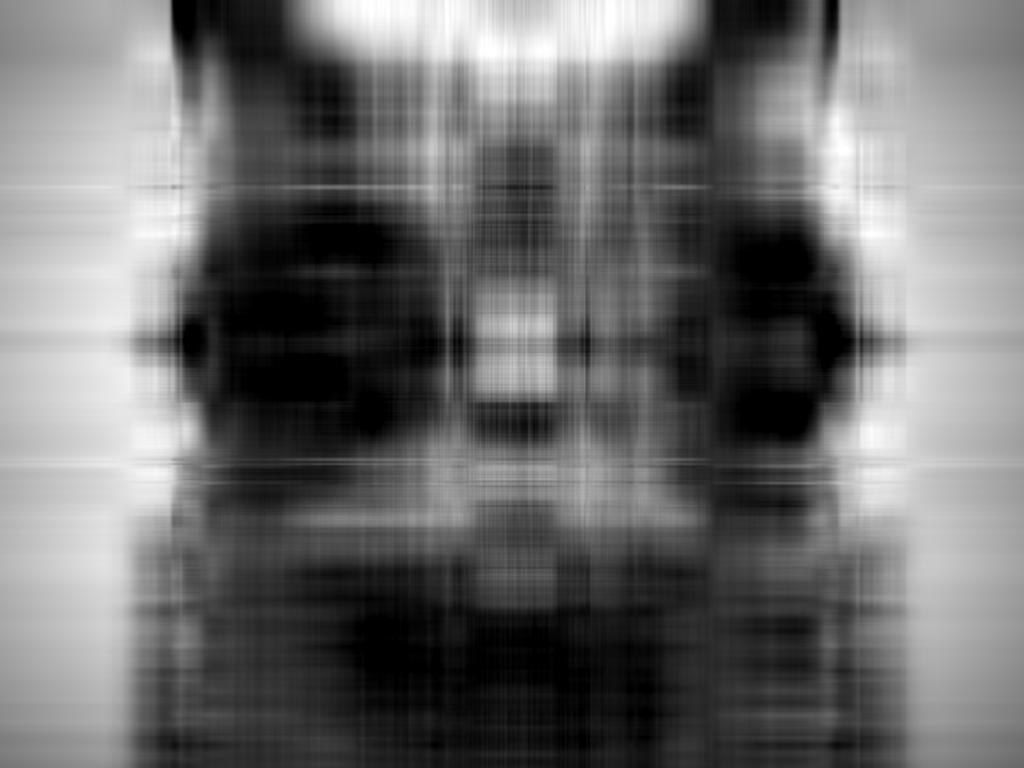
\includegraphics[width=.9\linewidth]{images/cat5}
\subcaption{SW $\sigma_1,\ldots, \sigma_5$.}
\end{subfigure}
\begin{subfigure}[c]{.3\textwidth}
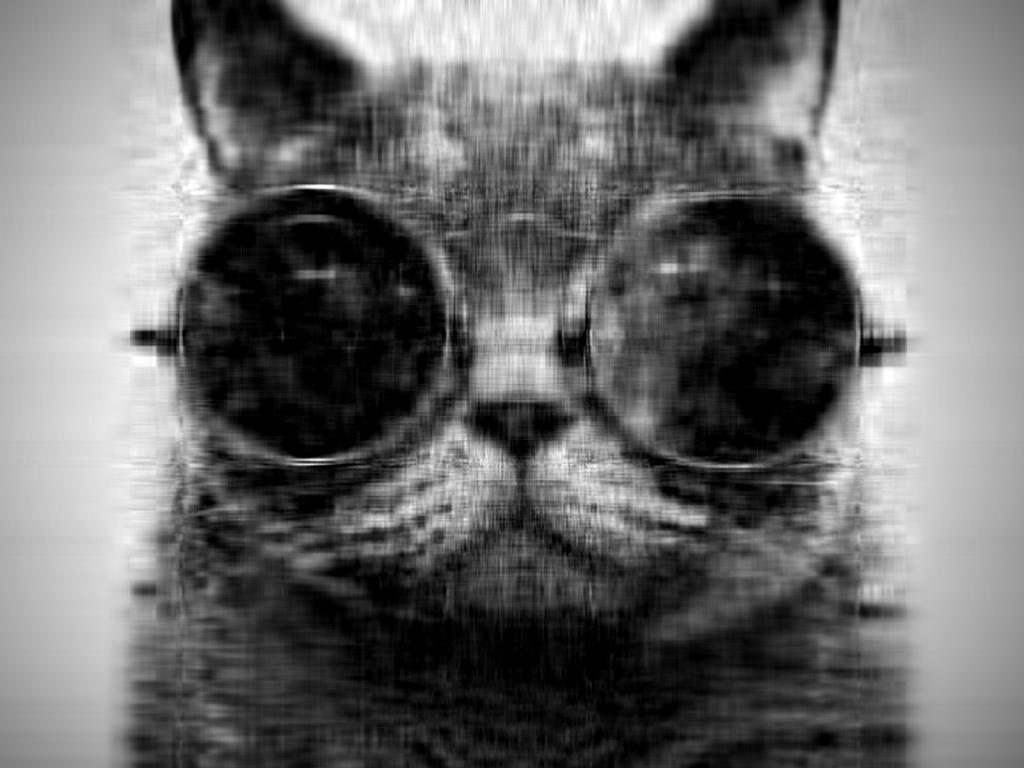
\includegraphics[width=.9\linewidth]{images/cat20}
\subcaption{SW $\sigma_1,\ldots, \sigma_{20}$.}
\end{subfigure}

\vspace{0.4cm}
\begin{subfigure}[c]{.3\textwidth}

\includegraphics[width=.9\linewidth]{images/cat50}
\subcaption{SW $\sigma_1,\ldots, \sigma_{50}$.}
\end{subfigure}
\begin{subfigure}[c]{.3\textwidth}

\includegraphics[width=.9\linewidth]{images/cat100}
\subcaption{SW $\sigma_1,\ldots, \sigma_{100}$.}
\end{subfigure}
\begin{subfigure}[c]{.3\textwidth}

\includegraphics[width=.9\linewidth]{images/cat300}
\subcaption{SW $\sigma_1,\ldots, \sigma_{300}$.}
\end{subfigure}

\caption{Approximation von Abbildung \ref{im:cat} mittels Singul"arwertzerlegung.}
\end{figure}

Dieser Versuch wirkt "uberzeugender. Bereits bei Figur (e) ist ein genauer Blick erforderlich, um die Makel der Komprimierung zu erkennen.
Bei der Verwendung der ersten 300 SW ist es nahezu unm"oglich einen Unterschied zum Original festzustellen.
Es ist also zu "uberlegen, ob man sich mit der Qualit"at der Figur (f) zufrieden geben m"ochte und statt Abbildung \ref{im:cat} nicht einfach dieses abspeichert.\\

Das Approximieren von Bildern ist ein sehr spezieller Fall des Filterns von Eigenwerten und die Berechnung der Singul"arwertzerlegung nicht immer zweckm"a"sig oder m"oglich.
Daher setzt sich diese Arbeit mit Alternativen auseinander, die dem Filtern dienlich sind. Das Ziel dabei ist neben der mathematischen Herleitung dieser Alternativen \textcolor{red}{und weiter?}%auch das Sensibilisieren

%Doch bevor es konkreter wird, soll der folgende Abschnitt ein Fundament erschaffen, das es erm"oglicht, den Gedankeng"angen dieser Arbeit besser folgen zu k"onnen.

\section{Mathematische Grundlagen}

Um das Lesen dieser Arbeit mehr zu einer Freude denn zu einer Schikane zu
machen, soll dieser Abschnitt ein mathematisches Fundament erschaffen, das es erm"oglicht, den Gedankeng"angen dieser Schrift besser folgen zu k"onnen.
Obschon sich der Autor bem"uht hat,
in der Literatur g"angige Notation zu benutzen, bittet er den
verst"andnisvollen Leser bei Unklarheiten im Anhang A nachzuschlagen.\\

Mit den Buchstaben $m$ und $n$ werden wir -- sofern nicht anders vermerkt -- zwei nat"urliche Zahlen bezeichnen. Dabei wollen wir die Null aus den nat"urlichen Zahlen $\N$ ausgeschlossen wissen.
Falls die Null zugelassen ist, schreiben wir explizit $\N_0 := \N\cup\{0\}$. Des Weiteren werden wir,
in Anlehnung an die in \emph{MATLAB} verwendete Syntax, Gebrauch von der Notation $i=m:n$ an Stelle von $i=m,m+1,\ldots,n-1,n$ machen.
Diese Kurzschreibweise wird etwa bei der Einf"uhrung von Indizierungen zum Einsatz kommen.\\

Es sei nun $A$ eine quadratische, komplexwertige Matrix, also $A\in\Cnn$. Diese wird als \emph{hermitesch} bezeichnet, falls sie die Identit"at $A=A^H$ erf"ullt und ist \emph{positiv definit}, sofern
f"ur alle Vektoren $x\in\Co$ die Absch"atzung
\[
x^H A x > 0
\]
gilt. Folglich werden wir eine Matrix \emph{hermitesch positiv definit} (HPD)
nennen, wenn sie sowohl hermitesch als auch positiv definit ist. Sollte $A$ solch eine HPD-Martrix sein,
dann nennen wir eine Menge von Vektoren $\{x_k\}_{k=1:m}\subseteq\Cn$ \emph{orthonormal
bez"uglich} $A$ oder schlicht: \emph{$A$-orthonormal}, falls
f"ur alle $i,j = 1:m$
\[
x_i^H A x_j = \delta_{i,j} := \begin{cases}
1 & \text{ wenn } i=j \\
0 & \text{ wenn } i\neq j
\end{cases}
\]
gilt. Allgemeiner hei"st eine Matrix $X\in\Cnn$ \emph{orthogonal bez"uglich} $A$ oder \emph{$A$-orthogonal}, falls sie
\[
X^H A X = I_n
\]
erf"ullt. Aus der Hermitizit"at von $A$ und $I_n$ folgt nat"urlich ebenfalls $XAX^H = I_n$. F"ur den Fall $A=I_n$ ignorieren wir in der Formulierung den Bezug zu $A$ und sprechen lediglich von Orthogonalit"at beziehungsweise Orthonormalit"at.\\

Sei im Folgenden $A$ wieder eine beliebige komplexwertige Matrix. Neben dieser betrachten wir nun noch eine weitere Matrix $B\in\Cnn$.
Unter einem \emph{$n$-dimensionalen Eigenwertproblem} wollen wir die Aufgabe verstehen, Paare $(\lambda,x)\in\C\times\Co$ zu finden, die der Gleichung
\begin{equation}\label{eq:chap1:evp}
Ax = \lambda Bx
\end{equation}
gen"ugen. Wenn klar ist, dass von solch einem Problem die Redes ist, werden wir anstelle des Wortes \glqq Eigenwertproblem\grqq\ die Notation $(A,B)$ als Bezeichnung verwenden und auf die Angabe der Dimension verzichten. Im Spezialfall $B=I_n$
hei"st $(A,B)$ \emph{gew"ohnliches Eigenwertproblem der Dimension $n$}.\\

Ist ein passendes Paar $(\lambda,x)$ gefunden, welches die \emph{Eigenwertgleichung} \eqref{eq:chap1:evp} l"ost, so nennen wir dieses \emph{Eigenpaar von} $(A,B)$ oder kurz: \emph{Eigenpaar}, falls bekannt ist, von welchem Eigenwertproblem die Rede ist.
Dabei hei"st $\lambda$ \emph{Eigenwert von} $(A,B)$ und $x$ \emph{Eigenvektor zum Eigenwert} $\lambda$ \emph{von} $(A,B)$. Auch hier werden wir auf die Angabe des Eigenwertproblems verzichten, wenn der Kontext dies gestattet.
Beim gew"ohnlichen Eigenwertproblem sehen wir von der Paar-Schreibweise ab und sprechen direkt von Eigenpaaren, Eigenwerten und Eigenvektoren von $A$.\\

Wie auf der Titelseite angek"undigt, wird sich diese Arbeit "uberwiegend mit der Behandlung \emph{hermitesch positiv definiter Eigenwertprobleme} (HPD-Eigenwertprobleme) befassen.
Damit seien f"urderhin Eigenwertprobleme $(A,B)$ bezeichnet, bei denen wir uns mit einer hermiteschen Matrix $A$ sowie einer HPD-Matrix $B$ konfrontiert sehen.\\

Eigenwertprobleme dieser Art besitzen eine Reihe n"utzlicher Eigenschaften, an denen wir uns zu einem sp"ateren Zeitpunkt in der Arbeit bedienen werden.
Von besonderer Bedeutung wird dabei das folgende Resultat sein.

\begin{thm}\label{thm:chap1:realEigenvalues}
Ist $(A,B)$ ein HPD-Eigenwertproblem der Dimension $n$, so sind alle zugeh"origen Eigenwerte reell.
Au"serdem existiert eine $B$-orthogonale Matrix $X\in\Cnn$ sowie eine Diagonalmatrix $\Lambda\in\R^{n,n}$ mit
\begin{equation}\label{eq:chap1:evpMatrix}
A = BX\Lambda X^{-1}.
\end{equation}
\end{thm}

\begin{proof}
Sei $(\lambda,x)$ ein Eigenpaar von $(A,B)$. Der positiven Definitheit von $B$ wegen, gilt nach Definition $x^H B x > 0$. Aus
\[
\lambda (x^H B x) = x^H Ax = x^H A^H x = (Ax)^H x
= \overline{\lambda} (Bx)^H x = \overline{\lambda} (x^H B x)
\]
folgt dann die Gleichheit $\lambda = \overline{\lambda}$ und somit $\lambda\in\R$.\\

 Um die Existenz der im Satz angegebenen Faktorisierung \eqref{eq:chap1:evpMatrix}
zu zeigen, ziehen wir unterst"utzend den Beweis aus ~\cite[Theorem 15.3.2, 344 f.]{parlett} zurate und erg"anzen diesen zur Vervollst"andigung durch weitere Argumente.
Zun"achst nutzen wir die Hermitizit"at und die positive Definitheit von $B$ aus. Mit diesen beiden Eigenschaften garantieren uns der Spektralsatz f"ur hermitesche Matrizen\footnote{Eine Formulierung mit/ohne Beweis ist im Anhang zu finden (Satz...).}
und der Satz von der Existenz der Cholesky-Zerlegung\footnote{Ebenfalls im Anhang zu finden.} eine Faktorisierung der Art
\begin{equation}\label{eq:chap1:factorization}
B = X_B \Lambda_B^2 X_B^H.
\end{equation}
Dabei ist $\Lambda_B\in\R^{n,n}$ eine diagonale Matrix und $X_B \in \C^{n,n}$ orthogonal.
Wir definieren uns nun eine weitere Matrix
\[
M:= \Lambda_B^{-1} X_B^H A X_B \Lambda_B^{-1},
\]
welche wegen
\[
M^H = \left(\Lambda_B^{-1} X_B^H A X_B \Lambda_B^{-1}\right)^H
= (\Lambda_B^{-1})^{H} X_B^H A^H (X_B^H)^H (\lambda_B^{-1})^H
= \Lambda_B^{-1} X_B^H A X_B \Lambda_B^{-1}
= M
\]
hermitesch ist. Erneut finden wir mit Hilfe des Spektralsatzes eine Zerlegung der Form
\[
M = X_M \Lambda_M X_M
\]
von $M$. Setzen wir nun $X:=X_M \Lambda_M X_M^H$, erhalten wir die Identit"aten
\begin{align*}
X^H A X &= X_M^H \Lambda_B^{-1} X_B^H A X_B \Lambda_B^{-1} X_M = X_M^H M X_M = \Lambda_M\\
X^H B X &= X_M^H \Lambda_B^{-1} X_B^H B X_B \Lambda_B^{-1} X_M \overset{\eqref{eq:chap1:factorization}}{=} X_M^H X_M = I_n.
\end{align*}
Also ist $X$ schon $B$-orthogonal. Schlie"slich folgt Gleichung \eqref{eq:chap1:evpMatrix} aus
\[
X^{-1}B^{-1}AX = X^{-1}B^{-1} (X^H)^{-1} X^H AX = \Lambda_M.
\]
durch Umstellen.
\end{proof}

Die Existenz der Faktorisierung \eqref{eq:chap1:factorization}
werden wir sp"ater nutzen, um bei HPD-Eigenwertproblem $(A,B)$ anstelle von \eqref{eq:chap1:evp} das L"osen von
\[
AX = BX\Lambda
\]
verlangen.






\begin{prop}
Ist $p$ eine Projektion auf den Unterraum $U$, dann gilt $p(u) = u$ f"ur
alle $u \in U$.
\end{prop}
\begin{proof}
Sei zun"achst $u \in \Bild{p}$. Dann existiert $v \in V$ mit $p(v) - u = 0$.
Nach Definition gilt aber auch $p^2(v)-u = p(u)-u = 0$. Also folgt $p(u)=u$.
\textcolor{red}{gilt $\Bild(p) = U$?}
\end{proof}

Bilinearit"at von $\langle \cdot, \cdot \rangle_A$
Kontur (komplex), Jordankurven, Invarianter Unterraum, Matrixpolynom\\

Eigenwertproblem $Ax = \lambda Bx$. Eigenpaare von $(A,B)$. Im Spezialfall $B=I$ kurz Eigenpaare von A.\\

Theorie zun"achst nicht auf hermitesche Probleme beschr"ankt oder doch? Jedenfalls einige Resultate f"ur hermitesche EWP\\

Schur-Vektoren $A = X\Lambda X^H$ sind die $x_i$.
